\documentclass[12pt,a4paper]{article}
\usepackage[mag=970, tikz]{newlistok}

\УвеличитьШирину{1.6cm}
\УвеличитьВысоту{2.6cm}
\renewcommand{\spacer}{\vspace{1.6pt}}

\ВключитьКолонтитул

\begin{document}

\Заголовок{Графы}
\НадНомеромЛистка{179 школа, 7Б.}
\Оценки{21/17/13}
\НомерЛистка{9}
\ДатаЛистка{18.11 -- 29.11/2017}


\СоздатьЗаголовок

\опр
\выд{Граф} задан, если задан конечный набор его \выд{вершин},
и для каждой пары разных вершин известно, связаны они \выд{ребром}
или нет (если связаны, эти вершины называются \выд{концами} этого ребра). Иногда граф удобно изображать как множество точек (вершин) на плоскости,
некоторые пары которых соединены линиями (рёбрами).
%(точки --- вершины, линии --- рёбра).
Бывают графы с \выд{кратными рёбрами}
(пару вершин могут соединять несколько рёбер) и \выд{петлями} (вершина может соединяться сама~с~собой).
%Ребро, соединяющее некоторую вершину саму с собой, называется
%\выд{петлёй}.\\ Рёбра, соединяющие одну и ту же пару вершин,
%называются \выд{параллельными} или \выд{кратными}.\\
%Граф, в котором нет петель и параллельных рёбер,
%называется \выд{простым}.\\
\копр

% \vspace*{-5mm}

\noindent
{\bf Примеры:} а) граф знакомств: вершины – школьники, рёбра – знакомства;
б) карта: вершины – страны, ребра – пары стран с общим участком границы; в) города и дороги;
г) граф короля (коня, ладьи, ферзя...): вершины – клетки, ребра – пары клеток, связанных одним ходом короля (коня, ладьи, ферзя...).



%\задача
%Про три компании, из шести человек каждая, известно следующее.
%Шестеро человек сели за круглый стол так, что знакомы были только сидящие рядом и напротив. Затем они пересели на две лавочки так, что на одной лавочке были незнакомые люди, а на разных --- знакомые.
%Каждый среди них знал троих, но среди любых трёх было хотя бы двое незнакомых.
%Могло ли такое быть?
%Могла ли это быть одна и та же компания?
%\кзадача


\пзадача
В шахматном турнире участвовали семь школьников. Известно, что Миша сыграл 6 партий, Коля -- 5, Илья и Гриша -- по три, Андрей и Сева -- по две, а Максим -- одну. С кем сыграл Илья?
\кзадача

\задача
\вСтрочку
\пункт
Идёт Петя,  а навстречу  ему 5 человек.
Докажите, что среди них найдутся либо трое,
знакомых с Петей, либо трое, незнакомых с Петей.
\пункт
Докажите, что среди любых 6 человек найдутся
либо 3 попарно знакомых, либо 3 попарно незнакомых человека.
\пункт
А если есть всего 5 человек?
\кзадача

\задача
Выпишите в ряд цифры 0, ..., 9 так, чтобы любые две соседние давали число, кратное 7~или~13.
\кзадача

% \задача
% В классе каждая девочка дружит с 5 мальчиками, каждый мальчик --- с 6 девочками. Кого больше?
% В графе каждая вершина синяя или белая. Каждая синяя вершина связана с 5-ю синими и 10-ю белыми, а каждая белая --- с 9-ю синими и 6-ю белыми. Каких вершин больше --- синих или белых?
% \кзадача
%

%\задача
%В углах доски $3\times3$ стоят кони: 2 белых (в соседних углах) и 2 чёрных. Можно ли за несколько шахматных ходов поставить их так, чтобы в любых двух соседних %углах кони были разного цвета?
%\кзадача

\опр
Два графа (без петель и кратных рёбер) называются \выд{изоморфными} (<<одинаковыми>>), если можно занумеровать вершины каждого графа одним и тем же набором различных номеров так, что %в графах получится один и тот же набор рёбер
будет выполнено условие:  если две вершины в первом графе соединены ребром, то и во втором графе вершины с этими же номерами соединены ребром, и наоборот.
%какие бы два номера не выбрать, ребро между вершинами с этими номерами либо есть в обоих графах, либо отсутствует в обоих графах.
%пара вершин в первом графа соединена ребром тогда и только тогда, когда пара вершин с такими же номерами во втором графе соединена ребром.
\копр

\УстановитьГраницы{0mm}{120mm}
%\rightpicture{-10mm}{1mm}{0.6}{isom}
\righttikz{-1mm}{0mm}{
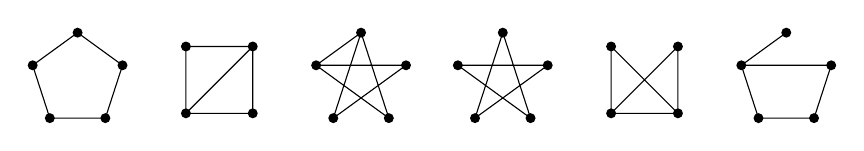
\begin{tikzpicture}[scale=.6]
\begin{scope}[xshift=0mm]
\coordinate (A) at (90:1);\coordinate (B) at (162:1);\coordinate (C) at (234:1);\coordinate (D) at (306:1);\coordinate (E) at (378:1);
\foreach \pt in {(A), (B), (C), (D), (E)} \fill \pt circle (3pt);
\draw (A)--(B)--(C)--(D)--(E)--(A);
\end{scope}
\begin{scope}[xshift=30mm]
\coordinate (A) at (45:1);\coordinate (B) at (135:1);\coordinate (C) at (225:1);\coordinate (D) at (-45:1);
\foreach \pt in {(A), (B), (C), (D)} \fill \pt circle (3pt);
\draw (A)--(B)--(C)--(D)--(A) (A)--(C);
\end{scope}
\begin{scope}[xshift=60mm]
\coordinate (A) at (90:1);\coordinate (B) at (162:1);\coordinate (C) at (234:1);\coordinate (D) at (306:1);\coordinate (E) at (378:1);
\foreach \pt in {(A), (B), (C), (D), (E)} \fill \pt circle (3pt);
\draw (A)--(B)--(D)--(A) (A)--(C)--(E)--(B);
\end{scope}
\begin{scope}[xshift=90mm]
\coordinate (A) at (90:1);\coordinate (B) at (162:1);\coordinate (C) at (234:1);\coordinate (D) at (306:1);\coordinate (E) at (378:1);
\foreach \pt in {(A), (B), (C), (D), (E)} \fill \pt circle (3pt);
\draw (A)--(C)--(E)--(B)--(D)--(A);
\end{scope}
\begin{scope}[xshift=120mm]
\coordinate (A) at (45:1);\coordinate (B) at (135:1);\coordinate (C) at (225:1);\coordinate (D) at (-45:1);
\foreach \pt in {(A), (B), (C), (D)} \fill \pt circle (3pt);
\draw (A)--(C)--(B)--(D)--(C)--(A)--(D);
\end{scope}
\begin{scope}[xshift=150mm]
\coordinate (A) at (90:1);\coordinate (B) at (162:1);\coordinate (C) at (234:1);\coordinate (D) at (306:1);\coordinate (E) at (378:1);
\foreach \pt in {(A), (B), (C), (D), (E)} \fill \pt circle (3pt);
\draw (A)--(B)--(C)--(D)--(E)--(B);
\end{scope}
\end{tikzpicture}
}
\задача
Разбейте графы, изображённые справа, на группы изоморфных.
\кзадача
\ВосстановитьГраницы





\УстановитьГраницы{0mm}{13cm}
\задача
Нарисуйте все неизоморфные друг другу графы с не более
чем четырьмя вершинами.
\кзадача
\ВосстановитьГраницы


%\УстановитьГраницы{0mm}{6.5cm}
% \rightpicture{-75mm}{15mm}{0.6}{isom-a}
% \rightpicture{-12mm}{15mm}{0.55}{isom-b}
\righttikz{-7mm}{15mm}{
\begin{tikzpicture}[scale=.5]
\node[above] at (-1,0) {\пункт};
\begin{scope}[xshift=0mm]
\coordinate (A) at (0,0);\coordinate (B) at (5,0);\coordinate (C) at (5,3);\coordinate (D) at (0,3);
\coordinate (AA) at (1.25,1);\coordinate (BB) at (3.75,1);\coordinate (CC) at (3.75,2);\coordinate (DD) at (1.25,2);
\foreach \pt in {(A), (B), (C), (D), (AA), (BB), (CC), (DD)} \fill \pt circle (3pt);
\draw (A)--(B)--(C)--(D)--(A) (AA)--(BB)--(CC)--(DD)--(AA) (A)--(AA) (D)--(DD);
\end{scope}
\begin{scope}[xshift=60mm]
\coordinate (A) at (0,0);\coordinate (B) at (5,0);\coordinate (C) at (5,3);\coordinate (D) at (0,3);
\coordinate (AA) at (1.25,1);\coordinate (BB) at (3.75,1);\coordinate (CC) at (3.75,2);\coordinate (DD) at (1.25,2);
\foreach \pt in {(A), (B), (C), (D), (AA), (BB), (CC), (DD)} \fill \pt circle (3pt);
\draw (A)--(B)--(C)--(D)--(A) (AA)--(BB)--(CC)--(DD)--(AA) (B)--(BB) (D)--(DD);
\end{scope}
\node[above] at (12,0) {\пункт};
\begin{scope}[xshift=150mm, yshift=17mm]
\coordinate (A) at (90:2); \coordinate (B) at (141:2); \coordinate (C) at (193:2); \coordinate (D) at (244:2); \coordinate (E) at (296:2); \coordinate (F) at (347:2); \coordinate (G) at (399:2);
\foreach \pt in {(A), (B), (C), (D), (E), (F), (G)} \fill \pt circle (3pt);
\draw (A)--(B)--(C)--(D)--(E)--(F)--(G)--(A) (A)--(C)--(E)--(G)--(B)--(D)--(F)--(A);
\end{scope}
\begin{scope}[xshift=210mm, yshift=17mm]
\coordinate (A) at (90:2); \coordinate (B) at (141:2); \coordinate (C) at (193:2); \coordinate (D) at (244:2); \coordinate (E) at (296:2); \coordinate (F) at (347:2); \coordinate (G) at (399:2);
\foreach \pt in {(A), (B), (C), (D), (E), (F), (G)} \fill \pt circle (3pt);
\draw (A)--(B)--(C)--(D)--(E)--(F)--(G)--(A) (A)--(D)--(G)--(C)--(F)--(B)--(E)--(A);
\end{scope}
\end{tikzpicture}}
\задача
Изоморфны ли графы:
% \пункт \hspace*{5.5cm}; \пункт \hspace*{5cm}.
\кзадача
%\ВосстановитьГраницы



\опр
\выд{Полный граф}\ --- граф, в котором каждые две разные вершины соединены одним ребром. %Полный граф с $n$ вершинами обозначается $K_n$.
\копр

\пзадача
Сколько рёбер в полном графе с $n$ вершинами? (Такой граф обозначается $K_n$.)
\кзадача

% \задача
%%В группе каждый мальчик дружит с 5-ю девочками, а каждая девочка --- с двумя мальчиками. Известно также, что для любых двух мальчиков есть ровно одна девочка,
%%которая дружит с обоими. Сколько
% В городе проводилось совещание врачей. От каждой поликлиники туда пригласили по 5 врачей. Оказалось, что каждый приглашенный работал в двух поликлиниках и на совещании представлял обе поликлиники. Кроме того, для любых двух поликлиник города среди участников совещания найдётся врач, который в них работает. Сколько в городе поликлиник и сколько врачей было на совещании?
% \кзадача

\задача
На листе даны \пункт 178; \пункт 179 точек. Играют двое: каждый в свой ход соединяет две точки линией. Нельзя соединять пару точек повторно. Проигрывает тот, после чьего хода из любой точки можно пройти в любую другую по линиям (и проходя их целиком). Кто может обеспечить себе победу?
\кзадача


\опр
\выд{Степень} ${\rm deg}\, V$ вершины $V$  ---  число
выходящих из неё рёбер (петли считаем~дважды).
\копр

% \задача
% У каждого из 179 марсиан три руки. Смогут ли они взяться за руки
% так, чтобы свободных рук не осталось? А если бы марсиан было 180?
% \кзадача

\задача
Сколько всего рёбер в графе \пункт ладьи; \пункт короля (на доске $8\times8$).
\кзадача

\vspace*{-1mm}
\пввзадача
\вСтрочку
%\пункт
%Можно ли соединить 77 телефонов между собой так,
%чтобы каждый был соединен ровно
%с 15 другими?
\пункт
Как связаны сумма степеней вершин любого графа
и количество его рёбер?\\
\пункт
Верно ли, что число вершин нечётной степени любого графа чётно?
\кзадача


\пзадача
В классе 27 ребят.
\пункт Докажите, что хотя бы двое из них имеют поровну друзей в классе.
\пункт Ученик Ян заметил: у остальных 26-ти разное число друзей
в классе. Сколько из них дружат~с~Яном?
\кзадача


% \задача
% На каждой из 100 карточек написано два целых числа (одно на одной стороне, другое --- на другой). Оказалось, что каждое целое число от 1 до 100 встречается среди написанных чисел дважды. Докажите, что карточки можно выложить в ряд так, что на видимых сторонах окажутся все целые числа от 1 до 100.
% \кзадача


\опр
\выд{Путь (длины $n$)}\ --- это последовательность вершин и соединяющих соседние вершины рёбер:
$V_1$, $e_1$, $V_2$, $e_2$, \dots, $e_n$, $V_{n+1}$. %Число $n$ называют \выд{длиной} пути.
Если $V_1=V_{n+1}$, путь называют \выд{циклическим},
а если и рёбра различны --- \выд{циклом}.
%, в~\hbox{которой} каж\-дые две соседние
%вершины соединены ребром.
%Последовательность рёбер $V_1 V_2$, $V_2V_3$, \dots, $V_n V_{n+1}$
%также называют путём.
Путь без повторяющихся рёбер --- \выд{цепь}, а без повторяющихся вершин --- \выд{простой путь}.
%а если ещё и вершины разные (кроме $V_1$ и $V_{n+1}$) ---
%\выд{простым циклом}.\\
%Граф называется \выд{связным}, если каждые две его вершины соединены путём.
\копр

\пзадача
Турист приехал на вокзал и пошёл гулять по улицам. Докажите, что он в любой момент~может вернуться на вокзал, проходя лишь те участки улиц, которые он уже прошёл нечётное~\hbox{число~раз.}
\кзадача


\опр
Граф называется \выд{связным}, если каждые две его вершины соединены путём.
\копр

\задача
В графе $n$ вершин, степень каждой не менее $\frac{n-1}{2}$. Докажите, что он связен.
\кзадача

\УстановитьГраницы{0mm}{3.5cm}
\rightpicture{-2.9mm}{6mm}{33mm}{koenig}
\задача %[Задача о кёнигсбергских мостах.]
Кёнигсберг располагался на берегах реки и 2-х островах, соединённых 7-ю мостами (см. рис.).
Можно ли было там прогуляться, %городу, %начав и закончив на центральном острове и
пройдя каждый мост ровно раз?
%\пункт А если начинать и заканчивать можно где угодно (не обязательно в одном и том же месте)?
\кзадача
\ВосстановитьГраницы

\пзадача [Эйлеровы графы]
Дан связный граф, степень любой его вершины чётна. Докажите,~что
\\\вСтрочку
\пункт в графе есть простой цикл;
\пункт рёбра графа можно разбить на циклы
(возможно, с общими вершинами, но без общих рёбер);
\пункт условие равносильно тому, что в графе есть цикл, содержащий все~рёбра.
\кзадача




\ЛичныйКондуит{0mm}{6mm}


\end{document}



\задача
В стране 2017 городов, каждый соединён
дорогами не менее, чем с 1008 другими.
Докажите, что из любого
города можно проехать в любой другой напрямую или
через один промежуточный город.
%\пункт найдутся 4 города, соединённые дорогами по циклу.
\кзадача

% \задача
% Группа островов соединена мостами.
%%так, что от каждого острова можно добраться до любого другого.
% Турист обошёл
% все острова, пройдя по каждому мосту %ровно
% один раз. На острове
% Светлом он побывал трижды. Сколько мостов ведёт со
% Светлого, если турист
% \вСтрочку
% \пункт
% не с него начал и не на нём закончил?
% \пункт
% с него начал, но не на нём закончил?
% \пункт
% с него начал и на нём закончил?
% \кзадача

\задача
Из столицы выходит 101 авиалиния, из
города Дальний --- одна, а из остальных городов по 100. Докажите,
что из столицы можно долететь в Дальний (возможно, с пересадками).
\кзадача


\задача
На какое наименьшее число частей надо разделить проволоку длиной 12 см, чтобы
из них можно было сделать каркас куба со стороной 1 см? Части можно %только
изгибать и скреплять друг с другом.
%Можно ли из куска проволоки длиной 120 см
%сделать каркас куба со стороной 10 см, не ломая проволоки?
\кзадача




% \задача
% \пункт Можно ли обойти всю шахматную доску конём по циклу?
% \пункт На шахматной доске стоит конь. Двое играют в игру, по очереди делая конём шахматный ход. Проиграет тот, кто поставит коня на клетку, где он уже был. Кто может обеспечить себе победу?
% \кзадача

\сзадача
% Известно, что в графе от любой вершины до любой другой можно добраться, пройдя суммарно не более 100 рёбер, а также можно добраться, пройдя суммарно чётное число рёбер (при подсчёте каждое ребро учитывается проходится несколько раз.
В~стране между некоторыми парами городов осуществляются двусторонние беспосадочные авиарейсы.
Известно, что из~любого города в~любой другой можно долететь, как сделав не~более 100 перелётов, так и сделав чётное число перелетов.
При каком наименьшем натуральном $d$ из~любого города можно гарантированно
долететь в~любой другой, сделав чётное число перелётов, не~превосходящее~$d$?
(Разрешается посещать один и~тот~же город или совершать один и~тот~же перелет
 более одного раза.)
\кзадача




% \задача
% \вСтрочку
% В некой стране $N$ городов, некоторые из которых соединены дорогами.
% Из любого города можно добраться в любой другой
% ровно одним способом (двигаясь по дорогам и нигде не разворачиваясь назад).
% \\
% \пункт Докажите, что в стране есть город, из которого ведёт ровно
% одна дорога.
% \пункт
% Сколько дорог в этой стране?
% \пункт
% Одну дорогу закрыли на ремонт. Можно ли теперь попасть из любого
% города в любой другой?
% \кзадача

ОРГРАФЫ

\опр
Граф называется \выд{ориентированным}, если на каждом ребре указано
направление.
%Пара вершин может при этом соединяться двумя рёбрами
%разных направлений.
\копр

\задача
В турнире каждая команда сыграла с каждой по разу.
Ничьих не было. Всегда ли можно расположить команды в таком
порядке, чтобы 1-я команда выиграла у 2-й,
2-я --- у 3-й, и т.~д.?
\кзадача

\задача
На новом сайте «Разговоры.ru» зарегистрировалось 2000 человек. Каждый из них пригласил к себе в друзья по 1000 человек. Два человека объявляются друзьями тогда и только тогда, когда каждый из них пригласил другого в друзья. Какое наименьшее количество пар друзей могло образоваться?
\кзадача


\задача
\вСтрочку
\пункт
Строка из 36 нулей и единиц начинается с 5 нулей.
Среди пятёрок подряд стоящих цифр~встречаются все 32 возможные комбинации.
Найти 5 последних цифр строки.
\пункт Почему такая строка есть?
\пункт ГИРЛЯНДЫ
\кзадача

\задача
Каждый из 450 депутатов дал пощёчину ровно одному своему
коллеге. Докажите, что из них можно выбрать 150
человек,  среди которых никто никому не давал пощёчины.
\кзадача

\сзадача
Схема проезда по городу представляет собой граф (рёбра --- улицы,
вершины --- перекрёстки). Назовём ребро $AB$ \выд{перешейком}, если
любой путь, соединяющий $A$ и $B$, содержит ребро $AB$.
%от $A$ до $B$ можно проехать единственным путём --- по ребру $AB$.
Докажите, что можно ввести на всех улицах, кроме перешейков, одностороннее
движение (а на перешейках --- двустороннее) так, чтобы от любого
перекрёстка можно было доехать по правилам до любого другого. %, не нарушая правил.
\кзадача

РАМСЕЙ

\задача
На плоскости отметили 17 точек и соединили каждые две из них
цветным отрезком: красным, желтым или зелёным.
Докажите, что
%\вСтрочку
%\пункт из каждой отмеченной точки
%выходит не меньше 6 одноцветных отрезков;
%\пункт
найдутся три точки в вершинах одноцветного треугольника.
\кзадача




\задача
У царя Гвидона было три сына (и больше детей не было).
Из его потомков сто имело по два сына, а остальные умерли бездетными.
Сколько потомков было у царя Гвидона?
\кзадача

%\vspace*{-5truemm}
\задача
%\вСтрочку
\пункт
На чаепитие пришли 27 школьников. Каждый принес по 2 пирожных.
Все пирожные раз\-ло\-жи\-ли на 27 тарелок (по 2 на тарелку).
Докажите, что, как бы ни были размещены пирожные,
можно так раздать тарелки школьникам, что каждому
достанется хотя бы одно пирожное, которое он сам принес.
\спункт  А если каждый принёс по 10 пирожных (и их разложили
по 10 штук на тарелку)?
\кзадача

\сзадача [Теорема Холла] В некоторой компании $n$ юношей.
При каждом $k$ от 1 до $n$ верно утверждение:
для любых $k$ юношей в компании число девушек,
знакомых хотя бы с одним из этих $k$ юношей, не меньше $k$.
Можно ли женить всех юношей на знакомых девушках?
\кзадача

